% 5-minute presentation of our project to the jury (Cybersecurity for NGOs Bootcamp, Training 3).
% Same theme as the training slides. Build from this folder: latexmk -lualatex 5-minute-presentation.tex
% Speaker notes (who says what, timing): change "hide notes" to "show notes on second screen=right".
\documentclass[aspectratio=169,11pt,t]{beamer}
\usetheme{focus}
\usepackage{qrcode}
\usetikzlibrary{arrows.meta}
\setbeameroption{hide notes}
\graphicspath{{screenshots/}}

% Shared look of the project presentations (5-minute-presentation.tex and project-overview.tex), next to the theme.
% ---- Background without the session progress bar (project presentations, not the training)
\makeatletter
\setbeamertemplate{background}{%
  \begin{tikzpicture}[x=1mm,y=1mm]
    \useasboundingbox (0,0) rectangle (160,90);
    \fill[paper] (0,0) rectangle (160,90);
    \fill[soft] (163,93) circle (26);
    \fill[soft!60] (139,96) circle (9);
    \fill[alert] (152,70) circle (1.4);
    \node[anchor=east, fill=white, rounded corners=3mm, inner xsep=3mm, inner ysep=1.6mm, font=\mediumfont\scriptsize, text=navy,
          blur shadow={shadow blur steps=6, shadow xshift=0, shadow yshift=-.3mm, shadow opacity=15}]
      at (148,80.5) {\textcolor{alert}{\faUserFriends}\ \insertframenumber\,/\,\inserttotalframenumber};
    % optional section tracker at the bottom (detailed deck): \sections{A,B,C} and \setsection{<n>}
    \ifdefined\pitch@sections
      \foreach \name [count=\i] in \pitch@sections {
        \pgfmathsetmacro\xa{12+(\i-1)*136/\pitch@nsec+.4}\pgfmathsetmacro\xb{12+\i*136/\pitch@nsec-.4}
        \ifnum\i=\pitch@cur \fill[alert, rounded corners=.4mm] (\xa,3.4) rectangle (\xb,4.8);
        \else\ifnum\i<\pitch@cur \fill[navy!70, rounded corners=.4mm] (\xa,3.7) rectangle (\xb,4.5);
        \else \fill[softdark!70, rounded corners=.4mm] (\xa,3.7) rectangle (\xb,4.5); \fi\fi
      }
    \fi
  \end{tikzpicture}}
\newcommand\sections[2]{\gdef\pitch@sections{#1}\gdef\pitch@nsec{#2}}
\newcount\pitch@cur
\newcommand\setsection[1]{\global\pitch@cur=#1\relax}
\makeatother

% ---- Helpers
% \screen[<width>]{<file>}: trainer-screen screenshot in a window frame (the app footer is cropped)
\newcommand\screen[2][\linewidth]{%
  \begin{tcolorbox}[enhanced, width=#1, arc=1.6mm, boxrule=.4pt, colframe=softdark, colback=white,
      left=0pt, right=0pt, top=0pt, bottom=0pt, before skip=0pt, after skip=0pt, drop fuzzy shadow={black!35}]
    \includegraphics[width=\linewidth, trim=0 215 0 0, clip]{#2}
  \end{tcolorbox}}
% \phone[<height>]{<file>}: phone screenshot in a phone frame (top part only)
\newcommand\phone[2][44mm]{%
  \tikz\node[inner sep=0pt, draw=ink, line width=1.1mm, rounded corners=3.5mm, fill=white, drop shadow={opacity=.25}]
    {\includegraphics[height=#1, trim=0 420 0 0, clip]{#2}};}
% \caption{<icon>}{<text>}
\newcommand\shotcaption[2]{{\scriptsize\color{muted}#1\ #2\par}}
% \point{<colour>}{<icon>}{<text>}: compact bullet card
\newcommand\point[3]{%
  \begin{card}[left=2.5mm, top=1.2mm, bottom=1.2mm, before skip=0pt, after skip=1.6mm]
    \iconbadge[6.5mm]{#1}{\small #2}\hspace{2.2mm}\begin{minipage}[c]{\dimexpr\linewidth-9mm\relax}\raggedright\mediumfont\footnotesize #3\end{minipage}
  \end{card}}
% \bigcard{<colour>}{<icon>}{<title>}{<text>}: card of the "why it works" slide
\newcommand\bigcard[4]{%
  \begin{card}[equal height group=why, before upper=\centering, left=2mm, right=2mm, top=2mm, bottom=2mm]
    \iconbadge[8mm]{#1}{#2}\par\vspace{1.2mm}
    {\headfont\small\color{navy}#3\par}\vspace{1mm}
    {\scriptsize\color{muted}#4\par}
  \end{card}}
\newcommand\stepbadge[3]{\tikz[baseline=(b.base)]\node[fill=#1, text=white, rounded corners=2mm, inner xsep=2.4mm, inner ysep=1.4mm, font=\headfont\small](b){#2\ #3};}



\title{When something goes wrong}

\begin{document}

% ---------- 1 · Title ----------
{\darkslide
\begin{frame}[plain,c]
  \vspace*{-2mm}
  {\kickerfont\fontsize{8}{10}\selectfont\color{alert}TRAINING 3 \textbullet{} OUR PROJECT}\par\vspace{4mm}
  \begin{minipage}{100mm}\raggedright
    {\headfont\fontsize{27}{32}\selectfont When something\\ goes wrong\par}\par\vspace{3mm}
    {\lightfont\fontsize{14}{18}\selectfont\color{soft}A simple incident response for NGOs,\\ in 60 minutes}\par\vspace{8mm}
    {\headfont\small\color{alert}\faFireExtinguisher\ Team Firefighters\par}\vspace{1.2mm}
    {\small\color{soft}Divya Ravichandran \textbullet{} Álvaro Gómez García\\Mohammed Krayem \textbullet{} University of Luxembourg\par}
  \end{minipage}
  \note{[15 s] "We are the Firefighters: Divya, Álvaro and Mohammed, cybersecurity students at the University of Luxembourg.
  Our training is Training 3: what to do when something goes wrong."}
\end{frame}
}

% ---------- 2 · The idea ----------
\begin{frame}{One analogy, one rule}{Our idea}
  \vspace{1mm}
  \begin{columns}[T,onlytextwidth]
    \column{.4\textwidth}
    \point{navy}{\faUsers}{\textbf{For:} NGO staff and volunteers with \textbf{no technical background}}
    \point{alert}{\faStopwatch}{\textbf{The problem:} the first minutes decide the damage, and most people don't know what to do}
    \point{good}{\faBullseye}{\textbf{Goal:} recognise an incident and take the right first steps}
    \column{.56\textwidth}
    \begin{card}[before upper=\centering, top=2.5mm, bottom=2.5mm]
      
\includegraphics[height=17mm]{firefighter}\par\vspace{.5mm}
      {\headfont\large\color{navy}An incident is like a fire\par}\vspace{.5mm}
      {\small\color{muted}the sooner you act, the less damage\par}\vspace{2.5mm}
      \stepbadge{alert}{1}{Stop}\hspace{.6mm}\stepbadge{navy}{2}{Disconnect}\par\vspace{1.2mm}
      \stepbadge{good}{3}{Report}\hspace{.6mm}\stepbadge{navydark}{4}{Write down}\par\vspace{2mm}
      {\scriptsize\color{muted}Never pay, delete or hide \textbullet{} no blame for reporting\par}
    \end{card}
  \end{columns}
  \note{[35 s] "Our audience has no technical background. When something goes wrong, the first minutes
  decide the damage, and most people either do nothing or the wrong thing. So we built the whole hour on one
  analogy: an incident is like a fire, and that is why our team is called the Firefighters. And one rule with four steps: Stop, Disconnect, Report, Write down.
  The same words appear in every challenge."}
\end{frame}

% ---------- 3 · The hour ----------
% \planpart{x}{y}{colour}{name}{icon}{minutes}{duration}{tag}{definition}: one card of the plan
\newcommand\planpart[9]{%
  \node[anchor=north west, inner sep=0pt] at (#1,#2) {\begin{tcolorbox}[enhanced, width=32mm, height=20mm, colback=white, colframe=white,
      arc=2mm, boxrule=0pt, left=2mm, right=1.4mm, top=1.4mm, bottom=.8mm, before skip=0pt, after skip=0pt,
      borderline west={1mm}{0pt}{#3}, drop fuzzy shadow={black!18}]
    \begin{tikzpicture}[baseline=(c.base)]\node[circle, fill=#3, text=white, minimum size=5.6mm, inner sep=0pt, font=\scriptsize](c){#5};\end{tikzpicture}\hspace{1.4mm}%
    \begin{minipage}[c]{19.5mm}\raggedright{\headfont\footnotesize\color{navy}#4\par}\vspace{-.2mm}{\headfont\fontsize{6.6}{8}\selectfont\color{#3}#6 \textbullet{} #7\par}\end{minipage}\par\vspace{1mm}
    {\raggedright\fontsize{6.2}{7.4}\selectfont\color{ink}\textbf{#8.} #9\par}
  \end{tcolorbox}};}
\begin{frame}{One hour, one thread}{The session, minute by minute}
  \vspace{3mm}\noindent
  \begin{tikzpicture}[x=1mm,y=1mm]
    \useasboundingbox (0,-48) rectangle (136,4);
    % proportional bar: 1 minute = 136/60 mm
    \foreach \s/\e/\c/\n in {0/5/muted/1,5/10/alert/2,10/18/navy/3,18/26/navy/4,26/41/alert/5,41/53/alert/6,53/56/alert/7,56/60/good/8} {
      \fill[\c, rounded corners=.8mm] ({\s*136/60+.3},0) rectangle ({\e*136/60-.3},4);
      \node[font=\headfont\fontsize{6.5}{6}\selectfont, text=white] at ({(\s+\e)/2*136/60},2) {\n};
    }
    \planpart{0}{-2.5}{muted}{Welcome}{\faHandshake}{0–5'}{5 min}{Slides}{Introductions, “Raise your hand if…”, agenda. Everyone scans the QR code.}
    \planpart{34.67}{-2.5}{alert}{Quiz}{\faQuestionCircle}{5–10'}{5 min}{Challenge 2, start}{5 real situations on the phone: what the group already knows.}
    \planpart{69.33}{-2.5}{navy}{Spot it}{\faSearch}{10–18'}{8 min}{Slides}{What an incident is, the fire analogy, the “Incident or not?” vote.}
    \planpart{104}{-2.5}{navy}{Act on it}{\faFirstAid}{18–26'}{8 min}{Slides}{One rule, four steps: Stop, Disconnect, Report, Write down. What never to do.}
    \planpart{0}{-25.5}{alert}{Game}{\faGamepad}{26–41'}{15 min}{Challenge 3}{“Put out the fire”: 4 rooms \texttimes{} 4 steps, one team fire that grows every second.}
    \planpart{34.67}{-25.5}{alert}{Case}{\faUsers}{41–53'}{12 min}{Challenge 4}{“The urgent payment”: a new case, alone, then in groups, then debrief.}
    \planpart{69.33}{-25.5}{alert}{Quiz again}{\faChartLine}{53–56'}{3 min}{Challenge 2, end}{The same 5 questions: before / after, per objective and per person.}
    \planpart{104}{-25.5}{good}{Close}{\faClipboardCheck}{56–60'}{4 min}{Challenge 5}{The one-page cheat sheet, key messages and feedback.}
  \end{tikzpicture}\par\vspace{2.5mm}
  \centering
  \pill{alert}{\faHandPointer\ 37 of 60 minutes: participants act}\hspace{1.5mm}%
  \pill{navy}{\faMobile*\ One QR code for the whole hour}
  \note{[30 s] "Here is the hour, in eight parts. Short explanations alternate with activities: in 37 of the 60
  minutes participants are doing something. They scan one QR code at the start and use it for the quiz, the
  game and the final quiz. Álvaro will show you the quiz and the game."}
\end{frame}

% ---------- 4 · Quiz ----------
\begin{frame}{The quiz: what would you do?}{Challenge 2 \textbullet{} learner assessment}
  \vspace{1mm}
  \begin{columns}[T,onlytextwidth]
    \column{.65\textwidth}
    \screen{quiz-host-question}\par\vspace{1.2mm}
    \shotcaption{\faDesktop}{Trainer screen: 5 real situations, 1 per learning objective}\vspace{2mm}
    \pill{navy}{\faRandom\ 4 options: real beliefs}\hspace{1mm}\pill{alert}{\faEyeSlash\ No answers shown yet}
    \column{.31\textwidth}
    \centering\phone[50mm]{quiz-phone-q1}\par\vspace{1.2mm}
    \shotcaption{\faMobile*}{Phone: no app, no account}
  \end{columns}
  \note{[35 s] "We built our own Kahoot-style web app. Participants scan the QR code, choose a nickname and
  answer on their phone: no app, no account, online or onsite. Five real situations, one per learning objective.
  The wrong options are not silly: they are what people really believe, like switching the computer off. At the
  start we do not show the right answers, because..."}
\end{frame}

% ---------- 5 · Before / after ----------
\begin{frame}{The same quiz at the end}{Challenge 2 \textbullet{} before / after}
  \vspace{1mm}
  \begin{columns}[T,onlytextwidth]
    \column{.65\textwidth}
    \screen{quiz-before-after}\par\vspace{1.2mm}
    \shotcaption{\faFlask}{Example with test data: right answers per objective, start vs end}\vspace{2mm}
    \pill{good}{\faChartLine\ Per objective and per person}\hspace{1mm}\pill{navy}{\faDownload\ CSV as evidence}
    \column{.31\textwidth}
    \centering\phone[50mm]{quiz-phone-progress}\par\vspace{1.2mm}
    \shotcaption{\faMobile*}{Your own progress}
  \end{columns}
  \note{[30 s] "...we ask exactly the same questions again at minute 53. The app compares both rounds per
  objective and per person, and every participant sees their own progress on the phone. So we don't just say
  people learned: we can show it, and download it."}
\end{frame}

% ---------- 6 · Game ----------
\begin{frame}{The game: put out the fire}{Challenge 3 \textbullet{} serious game}
  \vspace{1mm}
  \begin{columns}[T,onlytextwidth]
    \column{.65\textwidth}
    \screen{game-host-question}\par\vspace{1.2mm}
    \shotcaption{\faHome}{4 rooms \texttimes{} 4 steps \textbullet{} one team fire that grows every second}\vspace{2mm}
    \pill{navy}{\faTint\ Right move = water}\hspace{1mm}\pill{alert}{\faGasPump\ Trap card = petrol}
    \column{.31\textwidth}
    \centering\phone[50mm]{game-phone-hacker}\par\vspace{1.2mm}
    \shotcaption{\faBolt}{Surprise: a ``hacker''}
  \end{columns}
  \note{[35 s] "In the game, the analogy becomes the rule. Our NGO has four rooms, each with a real
  incident, and each room is played in four phases: the four steps. The fire grows every second, a right move
  is water, and a classic mistake is a trap card: petrol, for the whole team. And in the last room, a fake
  manager sends a message: pay and keep it secret."}
\end{frame}

% ---------- 7 · Game evidence ----------
\begin{frame}{Every answer changes the fire}{Challenge 3 \textbullet{} feedback and evidence}
  \vspace{2mm}
  \begin{columns}[T,onlytextwidth]
    \column{.49\textwidth}
    \screen{game-host-reveal}\par\vspace{1.2mm}
    \shotcaption{\faCommentDots}{After each phase: answers, effect on the fire (waiting, water, petrol) and why}
    \column{.49\textwidth}
    \screen{game-debrief}\par\vspace{1.2mm}
    \shotcaption{\faChartBar}{Debrief: right moves per objective next to the quiz at the start, most chosen trap cards}
  \end{columns}
  \vspace{4mm}
  \centering\pill{good}{\faEye\ The trainer sees which misconceptions remain}\hspace{1mm}\pill{navy}{\faDownload\ CSV per person}
  \note{[30 s] "After every phase the screen shows what the team chose, how the fire changed, and why;
  each phone says Water or Petrol. At the end the trainer gets the right moves per objective, next to the quiz
  result at the start, and the trap cards people still fall for."}
\end{frame}

% ---------- 8 · Case ----------
\begin{frame}{The urgent payment}{Challenge 4 \textbullet{} learning by doing}
  \vspace{0mm}
  \begin{columns}[T,onlytextwidth]
    \column{.4\textwidth}
    \centering\tikz\node[inner sep=0pt, draw=softdark, line width=.3pt, drop shadow={opacity=.25}] {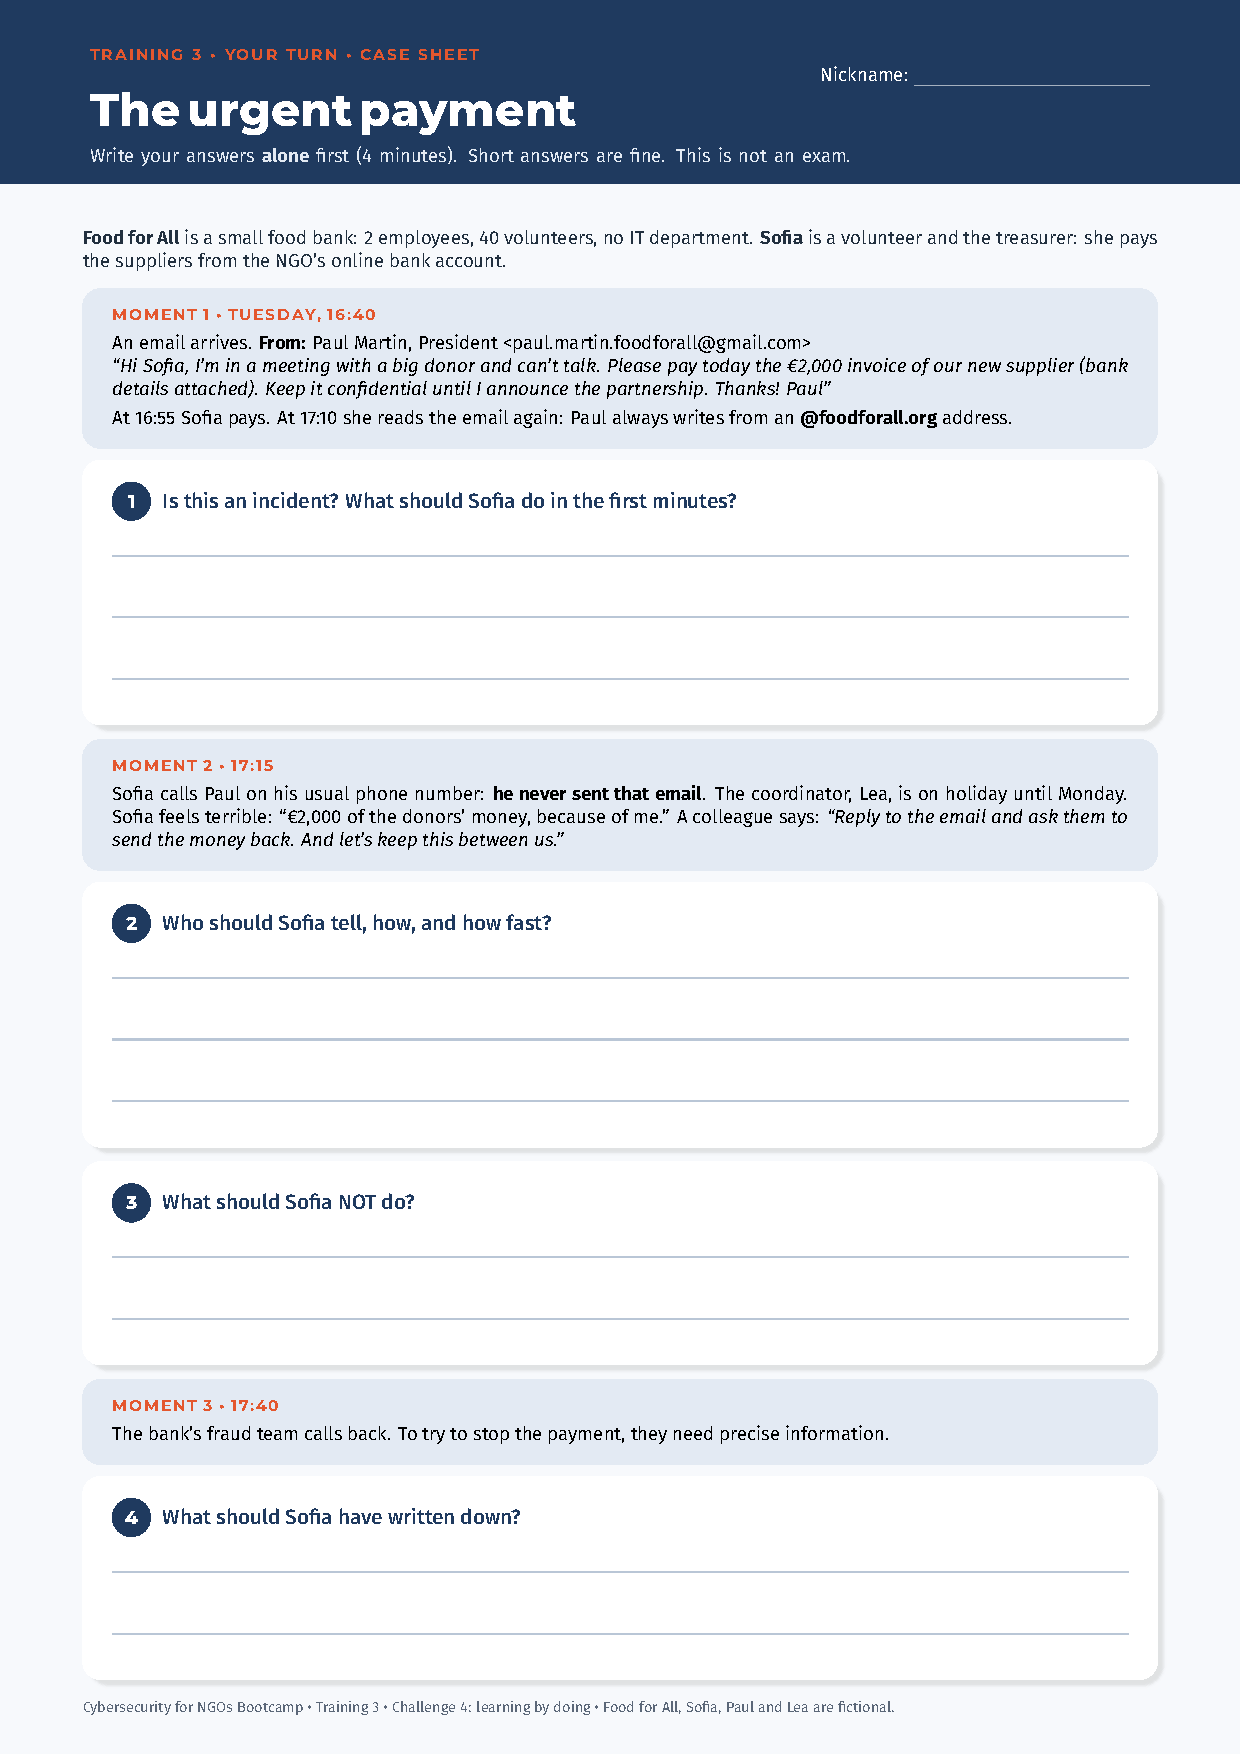
\includegraphics[height=60mm]{../04-learning-by-doing/case-sheet.pdf}};
    \column{.57\textwidth}
    \vspace{2mm}
    \point{alert}{\faEnvelope}{\textbf{A new case:} a fake email from the “president”, \textbf{€2,000} paid. No virus}
    \point{navy}{\faListOl}{\textbf{3 moments, 4 questions:} one per step of the rule}
    \point{good}{\faUsers}{\textbf{12'}: 4' alone \textrightarrow{} 4' groups \textrightarrow{} 4' debrief}
    \point{navydark}{\faClipboardCheck}{\textbf{Answer key:} good / partial / wrong, per objective}
    \vspace{.5mm}
    \pill{alert}{\faCheckCircle\ The real test: the rule on a new case}
  \end{columns}
  \note{[25 s] "Then each person applies the rule alone to a case they have never seen: a fake email from
  the president, and 2,000 euros paid. No virus, nothing broken: if they still stop, call the bank and report,
  they have understood the rule, not just memorised examples. Then they compare in groups, and we debrief."}
\end{frame}

% ---------- 9 · Cheat sheet ----------
\begin{frame}{The cheat sheet}{Challenge 5 \textbullet{} take-home}
  \vspace{0mm}
  \begin{columns}[T,onlytextwidth]
    \column{.4\textwidth}
    \centering\tikz\node[inner sep=0pt, draw=softdark, line width=.3pt, drop shadow={opacity=.25}] {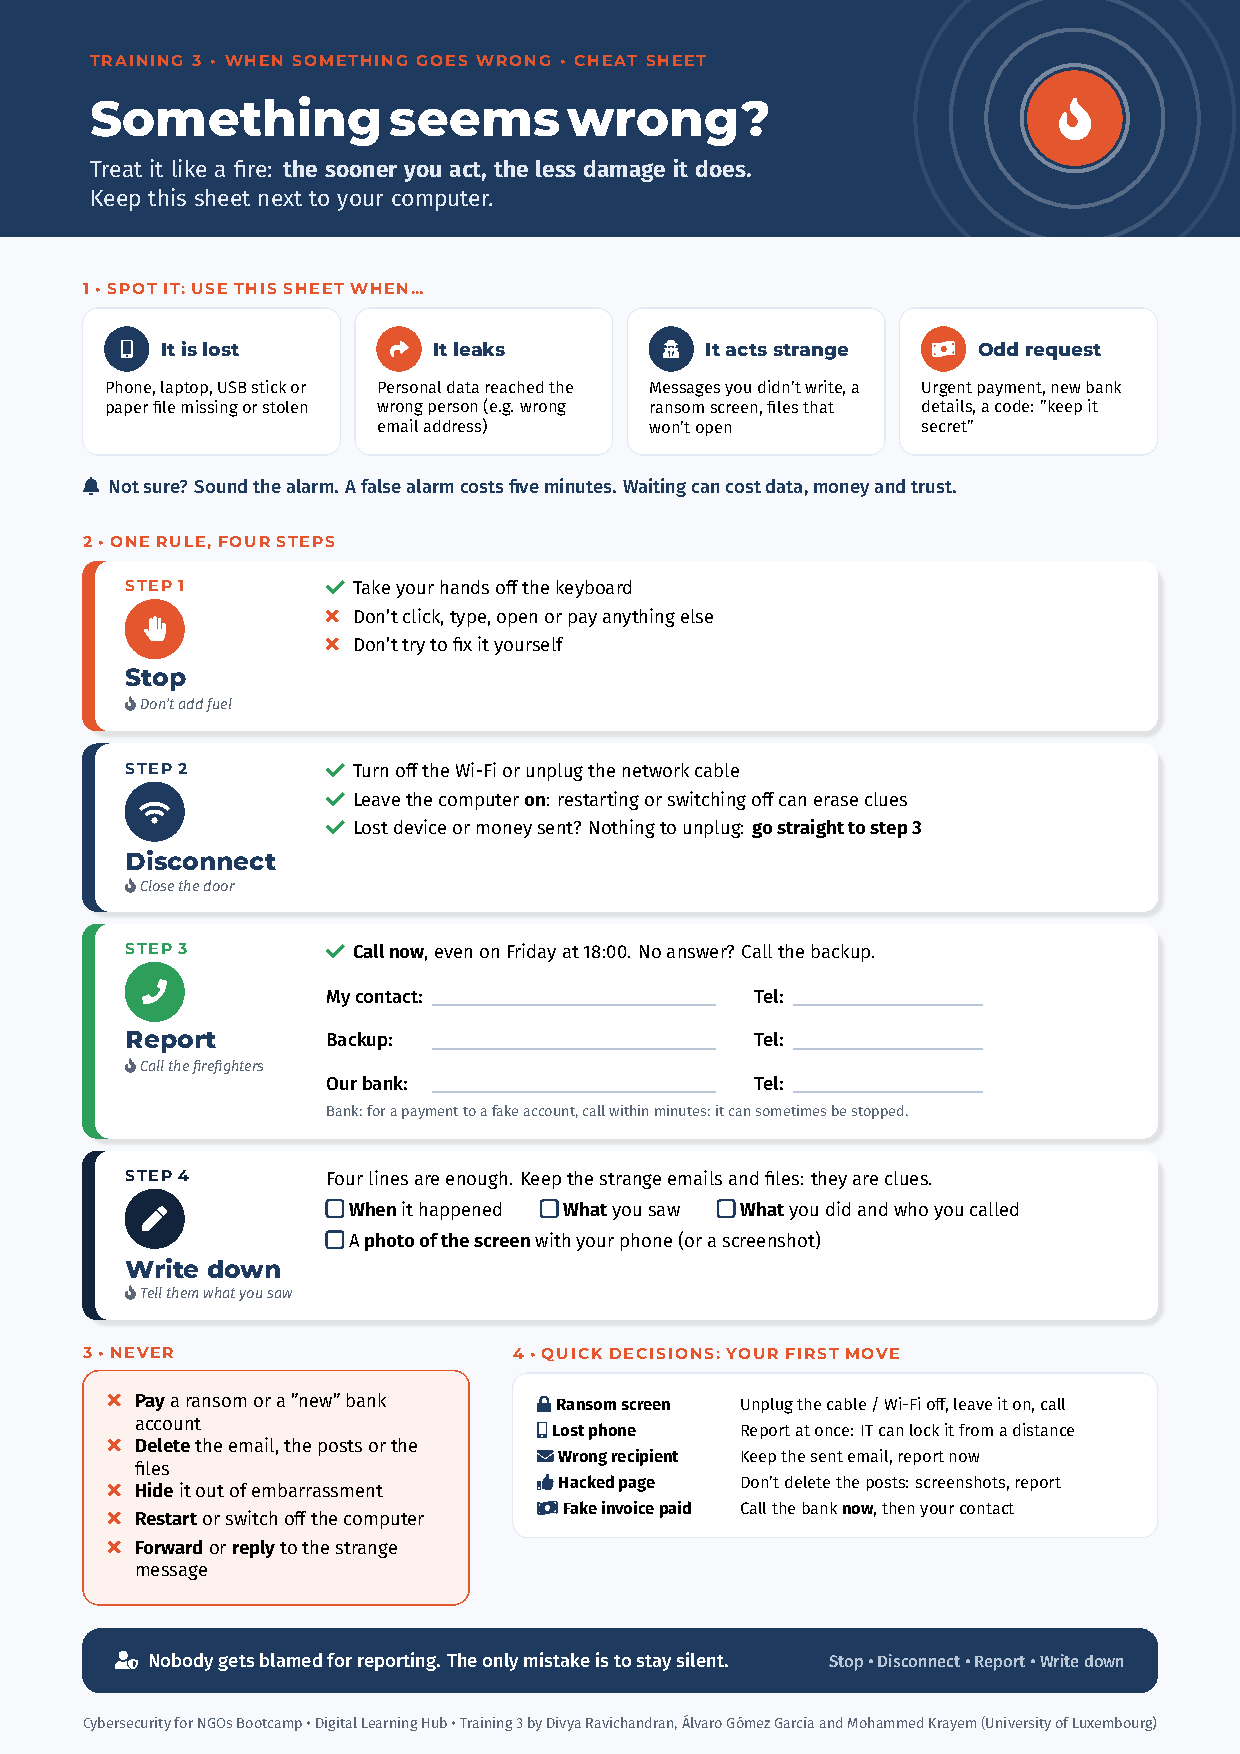
\includegraphics[height=60mm]{../05-take-home/cheat-sheet.pdf}};
    \column{.57\textwidth}
    \vspace{2mm}
    \point{alert}{\faExclamationTriangle}{\textbf{Spot it:} lost, leaks, acts strange, odd request}
    \point{navy}{\faListOl}{\textbf{The 4 steps:} what to do and not to do}
    \point{good}{\faPhone}{\textbf{Your phone numbers:} contact, backup, bank}
    \point{navydark}{\faBan}{\textbf{Never} list and \textbf{quick decisions} for 5 cases}
    \vspace{.5mm}
    \pill{navy}{\faThumbtack\ One page, to keep next to the computer}
  \end{columns}
  \note{[20 s] "And they leave with a one-page cheat sheet: when to use it, the four steps, what never to do,
  and their own contacts' phone numbers, written before they leave the room. In an emergency nobody looks for a number."}
\end{frame}

% ---------- 10 · Thank you ----------
{\darkslide
\begin{frame}[plain,c]
  {\kickerfont\fontsize{8}{10}\selectfont\color{alert}TRAINING 3 \textbullet{} WHEN SOMETHING GOES WRONG}\par\vspace{4mm}
  \begin{minipage}{112mm}\raggedright
    {\headfont\fontsize{30}{35}\selectfont Thank you!\par}\par\vspace{3mm}
    {\lightfont\fontsize{14}{18}\selectfont\color{soft}Stop \textbullet{} Disconnect \textbullet{} Report \textbullet{} Write down}\par\vspace{8mm}
    \pill{alert}{\faQuestionCircle\ Your questions}\hspace{1.5mm}%
    \pill{white!15!navy}{\faGithub\ github.com/algoga22/Focus-Activity-Training3}
  \end{minipage}
  \note{[5 s] "Thank you. We are happy to answer your questions." (Total about 5 minutes.)}
\end{frame}
}

\end{document}
